\section{Data and Sample}
\label{empirics}

\subsection{Conflict and City Data}

To measure economic performance we use annual percent change in GDP, which we collect from the World Development Indicators at the World Bank. We choose to focus on year over change in GDP because we expect conflicts proximate to major cities to lead to reductions in growth.\footnote{Alternative measures of economic performance would have included changes in FDI inflows or changes in GDP per capita, in using either of these measures are results remain relatively the same.} Unlike much of the extant literature in constructing our dependent variable we focus on year over change instead of a ten year average. We believe this approach to be superior because it allows us to estimate the direct effect of the conflict on economic performance in that year. A ten-year average approach might hide important variation in our dependent variable that can be explained by the proximity of conflict to economic centers.

Our key independent variable on the location of conflicts come from the PRIO Conflict Site Dataset. This dataset contains geo-referenced armed conflict events from 1989 to 2008.\footnote{We only include examine the effect of internal armed conflicts.} A downside of this geo-referenced database is that every conflict-year is assigned a circular conflict zone, which leads to the dataset reporting that the conflict is covering more territory than actually affected. Crafting a more specfic approach to the spread of conflict would, however, eliminate important cases from our analysis. In total this dataset provides us with almost 800 geo-referenced conflict-year cases. 

The key theory that we advance here is that the effects of conflict on economic performance are conditional on the proximity of those conflicts to major city centers. Thus a crucial part of our work here involved determining major city centers by year. The only data source we found with enough geographical and temporal coverage on major cities was The World Alamanac. To gather data from these textbooks we hired several undergraduate students to identify the major cities listed for each country within a yearly edition of the Almanac from 1989 to 2008. Major cities are classified as those that have relatively large shares of a country's population and/or are economic centers. Typically, the Alamanacs listed at least three major cities for each country and year from 1989 to 2008. After we had gathered a yearly list of major cities by country, we determined the centroid location of each city using Google's Geocoding API. 

In figure \ref{fig:CityConfMap}, we show the geographic distribution of conflicts and cities. The centroid locations of conflicts are shown by red dots. Not surprisingly, we can see that in many cases conflict locations are clustered within specific parts of a country. In most cases, this clustering is indicative of the same conflict moving within the geographic boundaries of a country over time. The blue diamonds in \ref{fig:CityConfMap} denote the locations of major cities as identified in The World Alamanacs from 1989 to 2008. Countries shaded in grey are those for which no armed conflict took place in this period according to the PRIO dataset.  

\begin{sidewaysfigure}[ht]
	\centering
	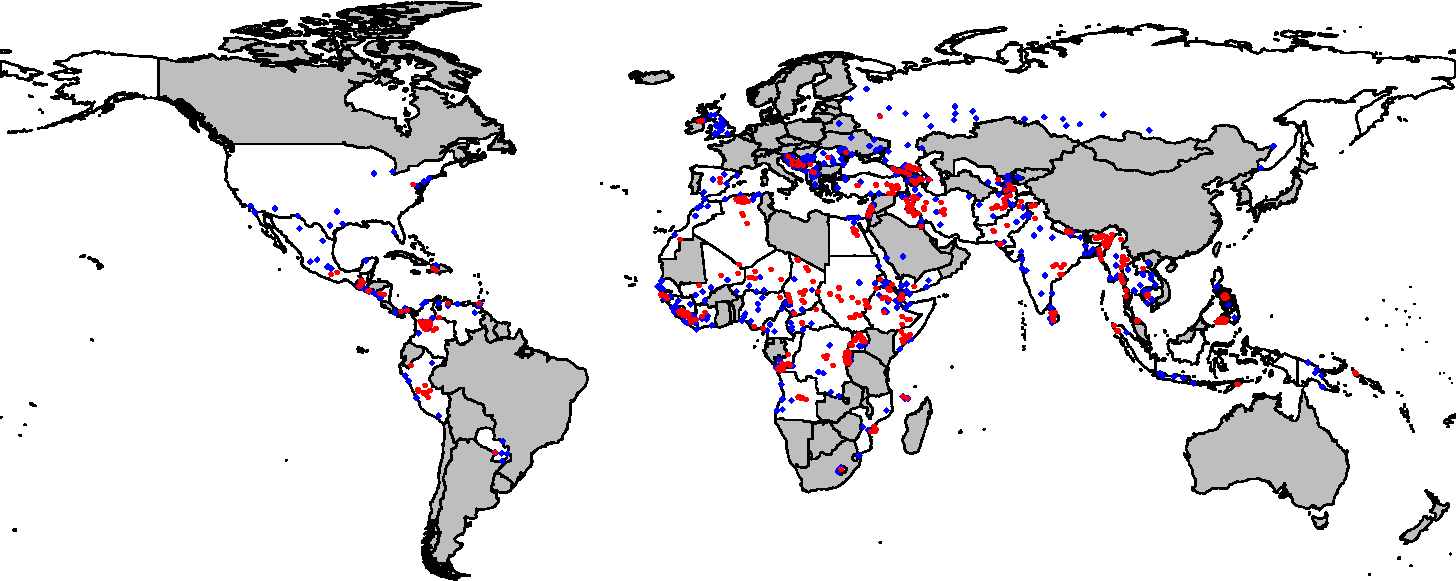
\includegraphics[width=.9\textwidth]{CityConfMap-crop}
	\caption{This map illustrates the geographic distribution of all conflicts, according to the PRIO Conflict Site Dataset, and major cities listed in The World Almanac from 1989 to 2008. Countries for which no armed conflicts are recorded are shaded in grey.}
	\label{fig:CityConfMap}
\end{sidewaysfigure}
\FloatBarrier

Our analysis focuses on exploring variations in economic growth in countries undergoing conflict by the proximity of those conflicts to major cities, thus we restrict our sample to only those countries that are listed as having conflicts in the PRIO dataset. To determine proximity, we calculate the distance in kilometers between the centroid of each of the conflicts with the centroids of city locations. Meaning that for each year we determine the distance between every conflict and every major city within a state. For example, in figure \ref{fig:columbiaMap} we show the location of armed conflicts in Colombia, dots colored in shades of red, and the major cities therein, blue diamonds.\footnote{One armed conflict involving rebel actors and the Colombian government occurred outside of Colombia's borders.} For Colombia each of the red dots represents the same conflict but a different year, with earlier years shaded in light red and later years shaded in dark red. Thus for every year we made six distance calculations -- one for every city.

\begin{figure}[ht]
	\centering
	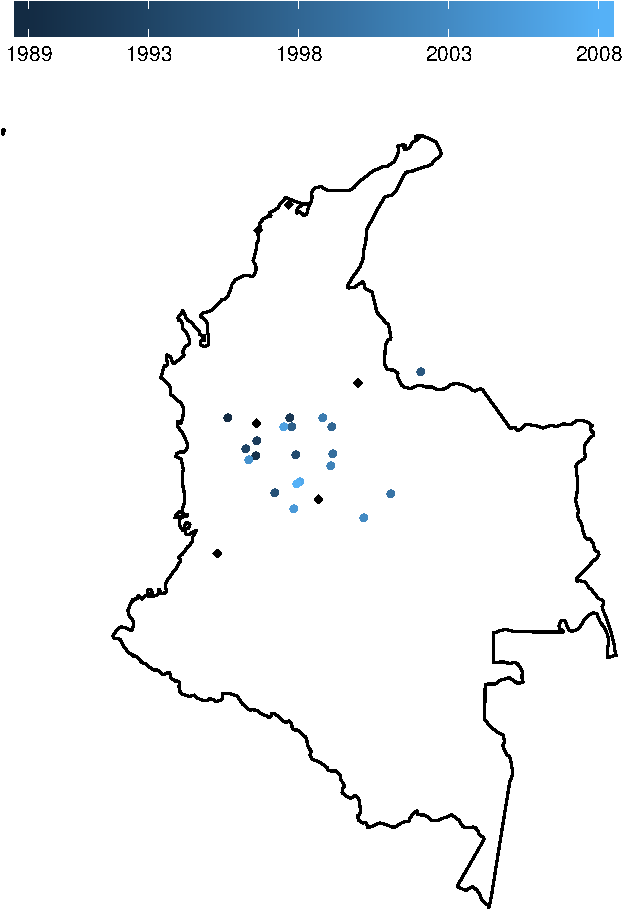
\includegraphics[width=.5\textwidth]{colombiaMap-crop}
	\caption{This map illustrates the geographic distribution of all conflicts, according to the PRIO Conflict Site Dataset, and major cities listed in The World Almanac from 1989 to 2008. Countries for which no armed conflicts are recorded are shaded in grey.}
	\label{fig:columbiaMap}
\end{figure}

\subsection{Level of Aggregation}

A key problem we face in conducting this analysis is reconciling the unit of analysis for our key independent and dependent variables. Our dependent variable is at the country-year and our key independent variable, distance between conflicts and major cities, is at the conflict-country-year level. To deal with this, we aggregate up to the country-year level by calculating the minimum logged distance any conflict is from a major city. Thus if a country faced, for example, four conflicts in one year, the datapoint that we would aggregate up to the country-year level would be for the conflict that was closest to a major city. This obviously is somewhat problematic as we end up discarding the information from the other conflicts. At the same time, we argue that this choice of aggregation is what conforms closest to our theoretical claims about economic activity only being severely disrupted in cases of conflicts being proximate to major cities. From the PRIO dataset we also bring in additional information about that conflict, specifically: 

\begin{itemize}
	\item Conflict intensity
	\item Ln(Conflict Area)
	\item Civil Conflict Type (e.g., territory or non-territory dispute)
	\item Conflict Duration (Years)
\end{itemize}

Last, we include a number of additional control measures. First, we control for a country's total, logged land area to differentiate between the proximity effects of conflicts within large and small countries. We also control for a couple of macroeconomic variables that could affect year over year changes in GDP, specifically, lagged inflation and whether or not the state is an upper income country, as defined by the World Bank.

\subsection{Estimation Method}

To estimate the model we use random effects clustered on countries and years. Results using a fixed effects estimation approach are similar.\footnote{The fixed effects model includes the same regressors as the random effects model but adds indicator variables for each country in the sample.}  The model we estimate is shown below:

\begin{align*}
	\% \Delta GDP_{i,t} &= \beta_{1}(Upper \; Income_{i,t}) \\
	& \;+\; \beta_{2}(Conflict \; Intensity_{i,t}) \;+\; \beta_{3}(Ln(Conflict \; Area)_{i,t}) \\
	& \;+\; \beta_{4}(Ln(Min. \; Conflict \; Dist.)_{i,t}) \;+\; \beta_{5}(Conflict \; Type_{i,t}) \\
	& \;+\; \beta_{6}(Conflict \; Duration_{i,t}) \;+\; \beta_{7}(Inflation_{i,t-1}) \\
	& \;+\; \beta_{8}(Ln(Land \; Area)_{i,t}) \;+\; \alpha_{i} + \gamma_{t} + \mu_{i,t}
\end{align*}

\section{Results}
\label{findings} 

We depict the results of our model in figure \ref{fig:coefPlot}. Most of the findings here are in line with our theoretical expectations. We find that higher levels of conflict intensity are associated with lower levels of GDP growth. The effect of conflict type is positive, indicating that non-territorial disputes are related to lower levels of GDP growth as well. Surprisingly, conflicts that are of a longer duration are, on average, not having a negative effect on GDP growth. 

Most importantly, we find strong support for our key hypothesis relating the proximity of a conflict to lower levels of GDP growth. The fact that the logged, minimum conflict distance variable is positive indicates that conflicts closer to major cities have an adverse effect on economic growth. 

\begin{figure}[ht]
	\centering
	\resizebox{.6\textwidth}{!}{% Created by tikzDevice version 0.6.2 on 2014-03-28 11:43:10
% !TEX encoding = UTF-8 Unicode
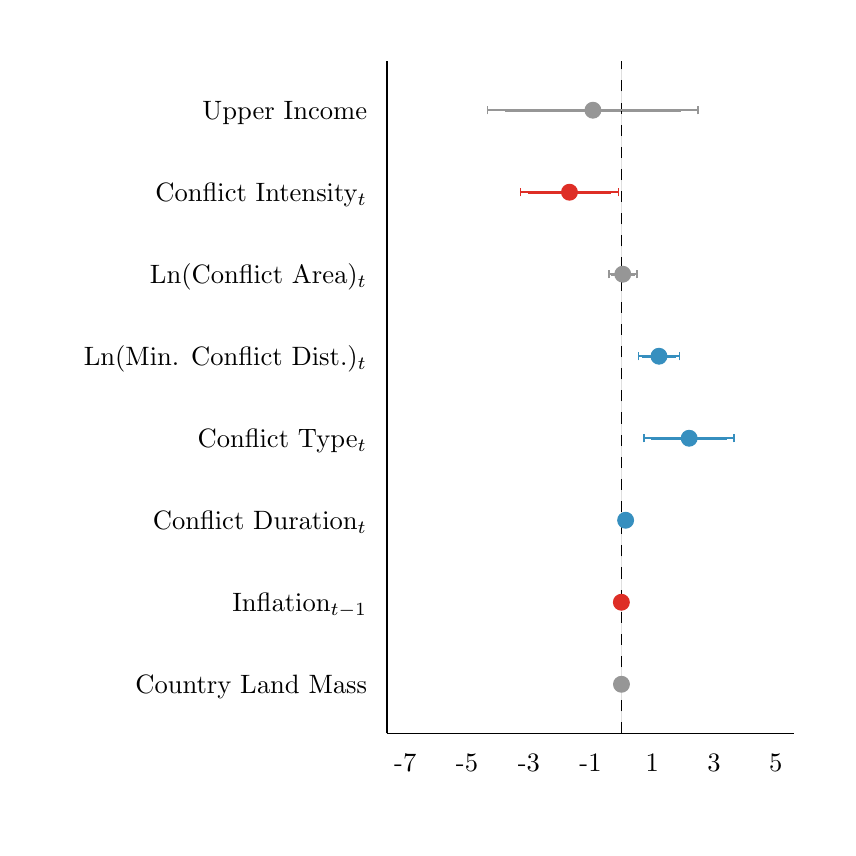
\begin{tikzpicture}[x=1pt,y=1pt]
\definecolor[named]{drawColor}{rgb}{0.00,0.00,0.00}
\definecolor[named]{fillColor}{rgb}{1.00,1.00,1.00}
\fill[color=fillColor,fill opacity=0.00,] (0,0) rectangle (289.08,289.08);
\begin{scope}
\path[clip] (  0.00,  0.00) rectangle (289.08,289.08);
\end{scope}
\begin{scope}
\path[clip] (  0.00,  0.00) rectangle (289.08,289.08);
\end{scope}
\begin{scope}
\path[clip] (  0.00,  0.00) rectangle (289.08,289.08);
\definecolor[named]{drawColor}{rgb}{1.00,1.00,1.00}
\definecolor[named]{fillColor}{rgb}{1.00,1.00,1.00}

\draw[color=drawColor,line width= 0.6pt,line cap=round,line join=round,fill=fillColor,] ( -0.00,  0.00) rectangle (289.08,289.08);
\end{scope}
\begin{scope}
\path[clip] (  0.00,  0.00) rectangle (289.08,289.08);
\end{scope}
\begin{scope}
\path[clip] (  0.00,  0.00) rectangle (289.08,289.08);
\end{scope}
\begin{scope}
\path[clip] (  0.00,  0.00) rectangle (289.08,289.08);
\end{scope}
\begin{scope}
\path[clip] (129.77, 34.03) rectangle (277.03,277.03);
\definecolor[named]{fillColor}{rgb}{1.00,1.00,1.00}

\draw[fill=fillColor,draw opacity=0.00,] (129.77, 34.03) rectangle (277.03,277.03);
\definecolor[named]{drawColor}{rgb}{0.59,0.59,0.59}
\definecolor[named]{fillColor}{rgb}{0.59,0.59,0.59}

\draw[color=drawColor,line width= 0.3pt,line join=round,fill=fillColor,fill opacity=0.30,draw opacity=0.30,] (214.56, 51.82) -- (214.56, 51.82);
\definecolor[named]{drawColor}{rgb}{0.87,0.18,0.15}
\definecolor[named]{fillColor}{rgb}{0.87,0.18,0.15}

\draw[color=drawColor,line width= 0.3pt,line join=round,fill=fillColor,fill opacity=0.30,draw opacity=0.30,] (214.52, 81.45) -- (214.54, 81.45);
\definecolor[named]{drawColor}{rgb}{0.21,0.56,0.75}
\definecolor[named]{fillColor}{rgb}{0.21,0.56,0.75}

\draw[color=drawColor,line width= 0.3pt,line join=round,fill=fillColor,fill opacity=0.30,draw opacity=0.30,] (215.47,111.08) -- (216.65,111.08);

\draw[color=drawColor,line width= 0.3pt,line join=round,fill=fillColor,fill opacity=0.30,draw opacity=0.30,] (222.76,140.72) -- (255.30,140.72);

\draw[color=drawColor,line width= 0.3pt,line join=round,fill=fillColor,fill opacity=0.30,draw opacity=0.30,] (220.66,170.35) -- (235.55,170.35);
\definecolor[named]{drawColor}{rgb}{0.59,0.59,0.59}
\definecolor[named]{fillColor}{rgb}{0.59,0.59,0.59}

\draw[color=drawColor,line width= 0.3pt,line join=round,fill=fillColor,fill opacity=0.30,draw opacity=0.30,] (209.97,199.99) -- (220.09,199.99);
\definecolor[named]{drawColor}{rgb}{0.87,0.18,0.15}
\definecolor[named]{fillColor}{rgb}{0.87,0.18,0.15}

\draw[color=drawColor,line width= 0.3pt,line join=round,fill=fillColor,fill opacity=0.30,draw opacity=0.30,] (178.06,229.62) -- (213.50,229.62);
\definecolor[named]{drawColor}{rgb}{0.59,0.59,0.59}
\definecolor[named]{fillColor}{rgb}{0.59,0.59,0.59}

\draw[color=drawColor,line width= 0.3pt,line join=round,fill=fillColor,fill opacity=0.30,draw opacity=0.30,] (166.20,259.25) -- (242.30,259.25);
\definecolor[named]{drawColor}{rgb}{0.59,0.59,0.59}
\definecolor[named]{fillColor}{rgb}{0.59,0.59,0.59}

\draw[color=drawColor,line width= 1.1pt,line join=round,fill=fillColor,] (214.56, 51.82) -- (214.56, 51.82);
\definecolor[named]{drawColor}{rgb}{0.87,0.18,0.15}
\definecolor[named]{fillColor}{rgb}{0.87,0.18,0.15}

\draw[color=drawColor,line width= 1.1pt,line join=round,fill=fillColor,] (214.52, 81.45) -- (214.53, 81.45);
\definecolor[named]{drawColor}{rgb}{0.21,0.56,0.75}
\definecolor[named]{fillColor}{rgb}{0.21,0.56,0.75}

\draw[color=drawColor,line width= 1.1pt,line join=round,fill=fillColor,] (215.57,111.08) -- (216.56,111.08);

\draw[color=drawColor,line width= 1.1pt,line join=round,fill=fillColor,] (225.38,140.72) -- (252.69,140.72);

\draw[color=drawColor,line width= 1.1pt,line join=round,fill=fillColor,] (221.86,170.35) -- (234.36,170.35);
\definecolor[named]{drawColor}{rgb}{0.59,0.59,0.59}
\definecolor[named]{fillColor}{rgb}{0.59,0.59,0.59}

\draw[color=drawColor,line width= 1.1pt,line join=round,fill=fillColor,] (210.79,199.99) -- (219.28,199.99);
\definecolor[named]{drawColor}{rgb}{0.87,0.18,0.15}
\definecolor[named]{fillColor}{rgb}{0.87,0.18,0.15}

\draw[color=drawColor,line width= 1.1pt,line join=round,fill=fillColor,] (180.91,229.62) -- (210.65,229.62);
\definecolor[named]{drawColor}{rgb}{0.59,0.59,0.59}
\definecolor[named]{fillColor}{rgb}{0.59,0.59,0.59}

\draw[color=drawColor,line width= 1.1pt,line join=round,fill=fillColor,] (172.32,259.25) -- (236.19,259.25);
\definecolor[named]{drawColor}{rgb}{0.00,0.00,0.00}
\definecolor[named]{fillColor}{rgb}{0.00,0.00,0.00}

\draw[color=drawColor,line width= 0.6pt,dash pattern=on 4pt off 4pt ,line join=round,fill=fillColor,] (214.56, 34.03) -- (214.56,277.03);
\definecolor[named]{drawColor}{rgb}{0.59,0.59,0.59}
\definecolor[named]{fillColor}{rgb}{0.59,0.59,0.59}

\draw[color=drawColor,line cap=round,line join=round,fill=fillColor,] (204.25,259.25) circle (  2.85);
\definecolor[named]{drawColor}{rgb}{0.87,0.18,0.15}
\definecolor[named]{fillColor}{rgb}{0.87,0.18,0.15}

\draw[color=drawColor,line cap=round,line join=round,fill=fillColor,] (195.78,229.62) circle (  2.85);
\definecolor[named]{drawColor}{rgb}{0.59,0.59,0.59}
\definecolor[named]{fillColor}{rgb}{0.59,0.59,0.59}

\draw[color=drawColor,line cap=round,line join=round,fill=fillColor,] (215.03,199.99) circle (  2.85);
\definecolor[named]{drawColor}{rgb}{0.21,0.56,0.75}
\definecolor[named]{fillColor}{rgb}{0.21,0.56,0.75}

\draw[color=drawColor,line cap=round,line join=round,fill=fillColor,] (228.11,170.35) circle (  2.85);

\draw[color=drawColor,line cap=round,line join=round,fill=fillColor,] (239.03,140.72) circle (  2.85);

\draw[color=drawColor,line cap=round,line join=round,fill=fillColor,] (216.06,111.08) circle (  2.85);
\definecolor[named]{drawColor}{rgb}{0.87,0.18,0.15}
\definecolor[named]{fillColor}{rgb}{0.87,0.18,0.15}

\draw[color=drawColor,line cap=round,line join=round,fill=fillColor,] (214.53, 81.45) circle (  2.85);
\definecolor[named]{drawColor}{rgb}{0.59,0.59,0.59}
\definecolor[named]{fillColor}{rgb}{0.59,0.59,0.59}

\draw[color=drawColor,line cap=round,line join=round,fill=fillColor,] (214.56, 51.82) circle (  2.85);

\draw[color=drawColor,line width= 0.6pt,line join=round,] (214.56, 50.33) --
	(214.56, 53.30);

\draw[color=drawColor,line width= 0.6pt,line join=round,] (214.56, 51.82) --
	(214.56, 51.82);

\draw[color=drawColor,line width= 0.6pt,line join=round,] (214.56, 50.33) --
	(214.56, 53.30);
\definecolor[named]{drawColor}{rgb}{0.87,0.18,0.15}
\definecolor[named]{fillColor}{rgb}{0.87,0.18,0.15}

\draw[color=drawColor,line width= 0.6pt,line join=round,] (214.54, 79.97) --
	(214.54, 82.93);

\draw[color=drawColor,line width= 0.6pt,line join=round,] (214.54, 81.45) --
	(214.52, 81.45);

\draw[color=drawColor,line width= 0.6pt,line join=round,] (214.52, 79.97) --
	(214.52, 82.93);
\definecolor[named]{drawColor}{rgb}{0.21,0.56,0.75}
\definecolor[named]{fillColor}{rgb}{0.21,0.56,0.75}

\draw[color=drawColor,line width= 0.6pt,line join=round,] (216.65,109.60) --
	(216.65,112.57);

\draw[color=drawColor,line width= 0.6pt,line join=round,] (216.65,111.08) --
	(215.47,111.08);

\draw[color=drawColor,line width= 0.6pt,line join=round,] (215.47,109.60) --
	(215.47,112.57);

\draw[color=drawColor,line width= 0.6pt,line join=round,] (255.30,139.24) --
	(255.30,142.20);

\draw[color=drawColor,line width= 0.6pt,line join=round,] (255.30,140.72) --
	(222.76,140.72);

\draw[color=drawColor,line width= 0.6pt,line join=round,] (222.76,139.24) --
	(222.76,142.20);

\draw[color=drawColor,line width= 0.6pt,line join=round,] (235.55,168.87) --
	(235.55,171.83);

\draw[color=drawColor,line width= 0.6pt,line join=round,] (235.55,170.35) --
	(220.66,170.35);

\draw[color=drawColor,line width= 0.6pt,line join=round,] (220.66,168.87) --
	(220.66,171.83);
\definecolor[named]{drawColor}{rgb}{0.59,0.59,0.59}
\definecolor[named]{fillColor}{rgb}{0.59,0.59,0.59}

\draw[color=drawColor,line width= 0.6pt,line join=round,] (220.09,198.50) --
	(220.09,201.47);

\draw[color=drawColor,line width= 0.6pt,line join=round,] (220.09,199.99) --
	(209.97,199.99);

\draw[color=drawColor,line width= 0.6pt,line join=round,] (209.97,198.50) --
	(209.97,201.47);
\definecolor[named]{drawColor}{rgb}{0.87,0.18,0.15}
\definecolor[named]{fillColor}{rgb}{0.87,0.18,0.15}

\draw[color=drawColor,line width= 0.6pt,line join=round,] (213.50,228.14) --
	(213.50,231.10);

\draw[color=drawColor,line width= 0.6pt,line join=round,] (213.50,229.62) --
	(178.06,229.62);

\draw[color=drawColor,line width= 0.6pt,line join=round,] (178.06,228.14) --
	(178.06,231.10);
\definecolor[named]{drawColor}{rgb}{0.59,0.59,0.59}
\definecolor[named]{fillColor}{rgb}{0.59,0.59,0.59}

\draw[color=drawColor,line width= 0.6pt,line join=round,] (242.30,257.77) --
	(242.30,260.74);

\draw[color=drawColor,line width= 0.6pt,line join=round,] (242.30,259.25) --
	(166.20,259.25);

\draw[color=drawColor,line width= 0.6pt,line join=round,] (166.20,257.77) --
	(166.20,260.74);
\end{scope}
\begin{scope}
\path[clip] (  0.00,  0.00) rectangle (289.08,289.08);
\end{scope}
\begin{scope}
\path[clip] (  0.00,  0.00) rectangle (289.08,289.08);
\definecolor[named]{drawColor}{rgb}{0.00,0.00,0.00}

\draw[color=drawColor,line width= 0.6pt,line join=round,fill opacity=0.00,] (129.77, 34.03) --
	(129.77,277.03);
\end{scope}
\begin{scope}
\path[clip] (  0.00,  0.00) rectangle (289.08,289.08);
\definecolor[named]{drawColor}{rgb}{0.00,0.00,0.00}

\node[color=drawColor,anchor=base east,inner sep=0pt, outer sep=0pt, scale=  0.96] at (122.65, 48.51) {Country Land Mass};

\node[color=drawColor,anchor=base east,inner sep=0pt, outer sep=0pt, scale=  0.96] at (122.65, 78.14) {Inflation$_{t-1}$};

\node[color=drawColor,anchor=base east,inner sep=0pt, outer sep=0pt, scale=  0.96] at (122.65,107.78) {Conflict Duration$_{t}$};

\node[color=drawColor,anchor=base east,inner sep=0pt, outer sep=0pt, scale=  0.96] at (122.65,137.41) {Conflict Type$_{t}$};

\node[color=drawColor,anchor=base east,inner sep=0pt, outer sep=0pt, scale=  0.96] at (122.65,167.05) {Ln(Min. Conflict Dist.)$_{t}$};

\node[color=drawColor,anchor=base east,inner sep=0pt, outer sep=0pt, scale=  0.96] at (122.65,196.68) {Ln(Conflict Area)$_{t}$};

\node[color=drawColor,anchor=base east,inner sep=0pt, outer sep=0pt, scale=  0.96] at (122.65,226.31) {Conflict Intensity$_{t}$};

\node[color=drawColor,anchor=base east,inner sep=0pt, outer sep=0pt, scale=  0.96] at (122.65,255.95) {Upper Income};
\end{scope}
\begin{scope}
\path[clip] (  0.00,  0.00) rectangle (289.08,289.08);
\end{scope}
\begin{scope}
\path[clip] (  0.00,  0.00) rectangle (289.08,289.08);
\end{scope}
\begin{scope}
\path[clip] (  0.00,  0.00) rectangle (289.08,289.08);
\end{scope}
\begin{scope}
\path[clip] (  0.00,  0.00) rectangle (289.08,289.08);
\end{scope}
\begin{scope}
\path[clip] (  0.00,  0.00) rectangle (289.08,289.08);
\end{scope}
\begin{scope}
\path[clip] (  0.00,  0.00) rectangle (289.08,289.08);
\end{scope}
\begin{scope}
\path[clip] (  0.00,  0.00) rectangle (289.08,289.08);
\definecolor[named]{drawColor}{rgb}{0.00,0.00,0.00}

\draw[color=drawColor,line width= 0.6pt,line join=round,fill opacity=0.00,] (129.77, 34.03) --
	(277.03, 34.03);
\end{scope}
\begin{scope}
\path[clip] (  0.00,  0.00) rectangle (289.08,289.08);
\end{scope}
\begin{scope}
\path[clip] (  0.00,  0.00) rectangle (289.08,289.08);
\end{scope}
\begin{scope}
\path[clip] (  0.00,  0.00) rectangle (289.08,289.08);
\definecolor[named]{drawColor}{rgb}{0.00,0.00,0.00}

\node[color=drawColor,anchor=base,inner sep=0pt, outer sep=0pt, scale=  0.96] at (136.46, 20.31) {-7};

\node[color=drawColor,anchor=base,inner sep=0pt, outer sep=0pt, scale=  0.96] at (158.77, 20.31) {-5};

\node[color=drawColor,anchor=base,inner sep=0pt, outer sep=0pt, scale=  0.96] at (181.09, 20.31) {-3};

\node[color=drawColor,anchor=base,inner sep=0pt, outer sep=0pt, scale=  0.96] at (203.40, 20.31) {-1};

\node[color=drawColor,anchor=base,inner sep=0pt, outer sep=0pt, scale=  0.96] at (225.71, 20.31) {1};

\node[color=drawColor,anchor=base,inner sep=0pt, outer sep=0pt, scale=  0.96] at (248.03, 20.31) {3};

\node[color=drawColor,anchor=base,inner sep=0pt, outer sep=0pt, scale=  0.96] at (270.34, 20.31) {5};
\end{scope}
\begin{scope}
\path[clip] (  0.00,  0.00) rectangle (289.08,289.08);
\end{scope}
\begin{scope}
\path[clip] (  0.00,  0.00) rectangle (289.08,289.08);
\end{scope}
\begin{scope}
\path[clip] (  0.00,  0.00) rectangle (289.08,289.08);
\end{scope}
\begin{scope}
\path[clip] (  0.00,  0.00) rectangle (289.08,289.08);
\end{scope}
\begin{scope}
\path[clip] (  0.00,  0.00) rectangle (289.08,289.08);
\end{scope}
\begin{scope}
\path[clip] (  0.00,  0.00) rectangle (289.08,289.08);
\end{scope}
\begin{scope}
\path[clip] (  0.00,  0.00) rectangle (289.08,289.08);
\end{scope}
\begin{scope}
\path[clip] (  0.00,  0.00) rectangle (289.08,289.08);
\end{scope}
\begin{scope}
\path[clip] (  0.00,  0.00) rectangle (289.08,289.08);
\end{scope}
\begin{scope}
\path[clip] (  0.00,  0.00) rectangle (289.08,289.08);
\end{scope}
\begin{scope}
\path[clip] (  0.00,  0.00) rectangle (289.08,289.08);
\end{scope}
\end{tikzpicture}
}
	\caption{Here we show the random effect regression results on GDP growth. Darker colors indicates that the coefficient estimate is significantly different from zero at a 95\% CI, while lighter the same for a 90\% CI. Grey indicates that the estimate is not significantly different from zero at either of those intervals.}
	\label{fig:coefPlot}	
\end{figure}
\FloatBarrier

To assess the substantive effect of the minimum conflict distance variable we conduct a number of simulations. We set up scenarios where we hold all variables to their median except for the logged, minimum conflict distance, which we range from its minimum to maximum value. Next, we conduct 1,000 random draws from a multivariate normal to obtain distributions for the point estimates of each of the regression coefficients. After obtaining these distributions, we calculate the predicted value of GDP growth based on the conditions set by the scenarios. We plot the results of this analyis in figure \ref{fig:simsPlot}.  

\begin{figure}[ht]
	\centering
	\resizebox{.8\textwidth}{!}{% Created by tikzDevice version 0.6.2 on 2014-03-28 19:46:55
% !TEX encoding = UTF-8 Unicode
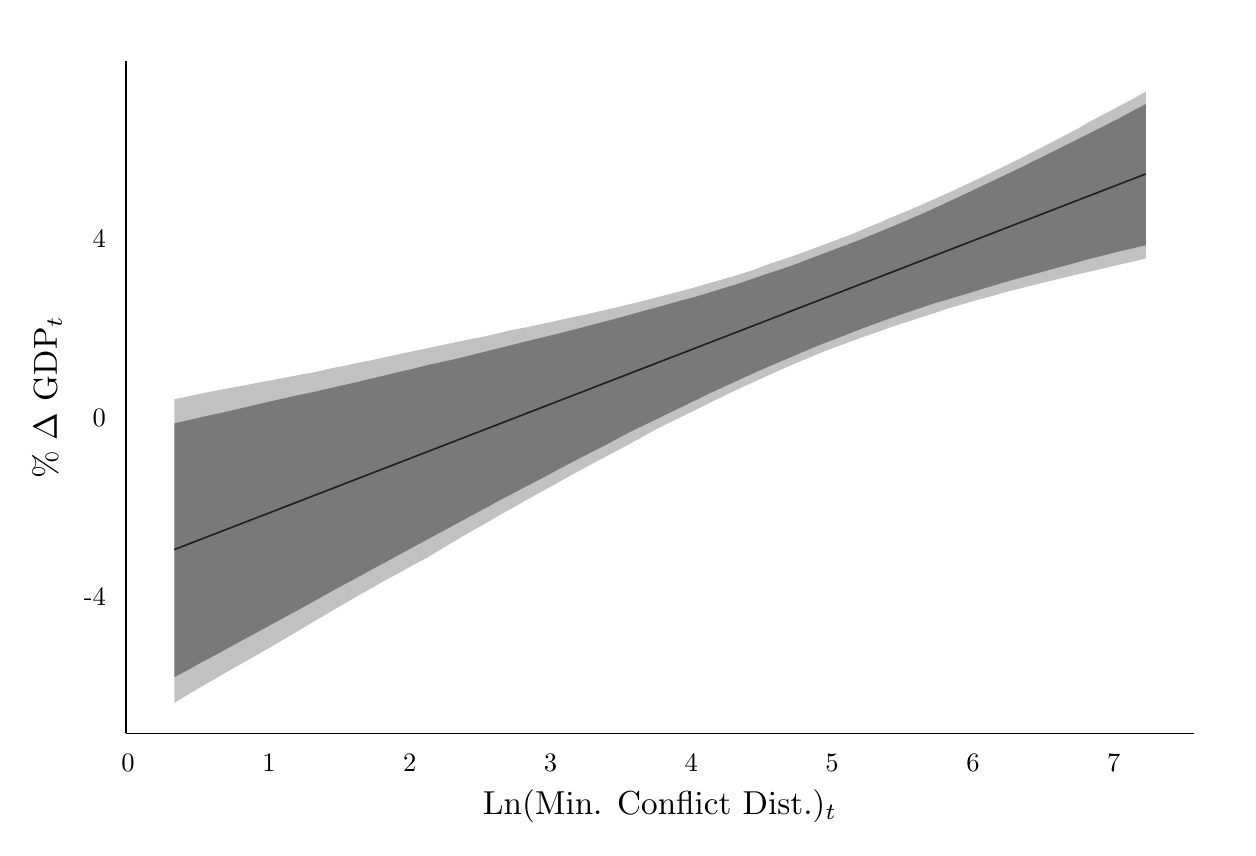
\begin{tikzpicture}[x=1pt,y=1pt]
\definecolor[named]{drawColor}{rgb}{0.00,0.00,0.00}
\definecolor[named]{fillColor}{rgb}{1.00,1.00,1.00}
\fill[color=fillColor,fill opacity=0.00,] (0,0) rectangle (433.62,289.08);
\begin{scope}
\path[clip] (  0.00,  0.00) rectangle (433.62,289.08);
\end{scope}
\begin{scope}
\path[clip] (  0.00,  0.00) rectangle (433.62,289.08);
\end{scope}
\begin{scope}
\path[clip] (  0.00,  0.00) rectangle (433.62,289.08);
\definecolor[named]{drawColor}{rgb}{1.00,1.00,1.00}
\definecolor[named]{fillColor}{rgb}{1.00,1.00,1.00}

\draw[color=drawColor,line width= 0.6pt,line cap=round,line join=round,fill=fillColor,] (  0.00,  0.00) rectangle (433.62,289.08);
\end{scope}
\begin{scope}
\path[clip] (  0.00,  0.00) rectangle (433.62,289.08);
\end{scope}
\begin{scope}
\path[clip] (  0.00,  0.00) rectangle (433.62,289.08);
\end{scope}
\begin{scope}
\path[clip] (  0.00,  0.00) rectangle (433.62,289.08);
\end{scope}
\begin{scope}
\path[clip] ( 35.42, 34.03) rectangle (421.57,277.03);
\definecolor[named]{fillColor}{rgb}{1.00,1.00,1.00}

\draw[fill=fillColor,draw opacity=0.00,] ( 35.42, 34.03) rectangle (421.57,277.03);
\definecolor[named]{drawColor}{rgb}{0.00,0.00,0.00}
\definecolor[named]{fillColor}{rgb}{0.00,0.00,0.00}

\draw[color=drawColor,line width= 0.6pt,line join=round,] ( 52.97,100.48) --
	( 58.06,102.45) --
	( 63.15,104.42) --
	( 68.24,106.39) --
	( 73.32,108.35) --
	( 78.41,110.32) --
	( 83.50,112.29) --
	( 88.59,114.25) --
	( 93.67,116.22) --
	( 98.76,118.19) --
	(103.85,120.16) --
	(108.94,122.12) --
	(114.03,124.09) --
	(119.11,126.06) --
	(124.20,128.02) --
	(129.29,129.99) --
	(134.38,131.96) --
	(139.46,133.93) --
	(144.55,135.89) --
	(149.64,137.86) --
	(154.73,139.83) --
	(159.81,141.80) --
	(164.90,143.76) --
	(169.99,145.73) --
	(175.08,147.70) --
	(180.17,149.66) --
	(185.25,151.63) --
	(190.34,153.60) --
	(195.43,155.57) --
	(200.52,157.53) --
	(205.60,159.50) --
	(210.69,161.47) --
	(215.78,163.43) --
	(220.87,165.40) --
	(225.95,167.37) --
	(231.04,169.34) --
	(236.13,171.30) --
	(241.22,173.27) --
	(246.30,175.24) --
	(251.39,177.20) --
	(256.48,179.17) --
	(261.57,181.14) --
	(266.66,183.11) --
	(271.74,185.07) --
	(276.83,187.04) --
	(281.92,189.01) --
	(287.01,190.98) --
	(292.09,192.94) --
	(297.18,194.91) --
	(302.27,196.88) --
	(307.36,198.84) --
	(312.44,200.81) --
	(317.53,202.78) --
	(322.62,204.75) --
	(327.71,206.71) --
	(332.80,208.68) --
	(337.88,210.65) --
	(342.97,212.61) --
	(348.06,214.58) --
	(353.15,216.55) --
	(358.23,218.52) --
	(363.32,220.48) --
	(368.41,222.45) --
	(373.50,224.42) --
	(378.58,226.39) --
	(383.67,228.35) --
	(388.76,230.32) --
	(393.85,232.29) --
	(398.93,234.25) --
	(404.02,236.22);
\definecolor[named]{fillColor}{rgb}{0.20,0.20,0.20}

\draw[fill=fillColor,fill opacity=0.30,draw opacity=0.00,] ( 52.97,154.81) --
	( 58.06,155.84) --
	( 63.15,156.96) --
	( 68.24,157.95) --
	( 73.32,158.93) --
	( 78.41,159.86) --
	( 83.50,160.85) --
	( 88.59,161.77) --
	( 93.67,162.75) --
	( 98.76,163.72) --
	(103.85,164.62) --
	(108.94,165.84) --
	(114.03,166.82) --
	(119.11,167.92) --
	(124.20,168.91) --
	(129.29,170.03) --
	(134.38,171.13) --
	(139.46,172.18) --
	(144.55,173.24) --
	(149.64,174.34) --
	(154.73,175.44) --
	(159.81,176.47) --
	(164.90,177.47) --
	(169.99,178.63) --
	(175.08,179.85) --
	(180.17,180.81) --
	(185.25,181.91) --
	(190.34,182.95) --
	(195.43,184.18) --
	(200.52,185.19) --
	(205.60,186.36) --
	(210.69,187.52) --
	(215.78,188.72) --
	(220.87,189.93) --
	(225.95,191.25) --
	(231.04,192.59) --
	(236.13,193.91) --
	(241.22,195.29) --
	(246.30,196.77) --
	(251.39,198.21) --
	(256.48,199.69) --
	(261.57,201.30) --
	(266.66,203.24) --
	(271.74,204.95) --
	(276.83,206.66) --
	(281.92,208.49) --
	(287.01,210.37) --
	(292.09,212.31) --
	(297.18,214.17) --
	(302.27,216.35) --
	(307.36,218.44) --
	(312.44,220.66) --
	(317.53,222.74) --
	(322.62,224.90) --
	(327.71,227.17) --
	(332.80,229.46) --
	(337.88,231.80) --
	(342.97,234.23) --
	(348.06,236.60) --
	(353.15,239.13) --
	(358.23,241.60) --
	(363.32,244.22) --
	(368.41,246.82) --
	(373.50,249.48) --
	(378.58,252.11) --
	(383.67,255.07) --
	(388.76,257.75) --
	(393.85,260.38) --
	(398.93,263.07) --
	(404.02,265.99) --
	(404.02,205.70) --
	(398.93,204.43) --
	(393.85,203.35) --
	(388.76,202.08) --
	(383.67,200.93) --
	(378.58,199.75) --
	(373.50,198.52) --
	(368.41,197.29) --
	(363.32,196.01) --
	(358.23,194.78) --
	(353.15,193.45) --
	(348.06,192.00) --
	(342.97,190.65) --
	(337.88,189.13) --
	(332.80,187.67) --
	(327.71,185.97) --
	(322.62,184.33) --
	(317.53,182.67) --
	(312.44,181.05) --
	(307.36,179.19) --
	(302.27,177.46) --
	(297.18,175.59) --
	(292.09,173.73) --
	(287.01,171.79) --
	(281.92,169.67) --
	(276.83,167.52) --
	(271.74,165.30) --
	(266.66,163.01) --
	(261.57,160.68) --
	(256.48,158.37) --
	(251.39,155.95) --
	(246.30,153.44) --
	(241.22,150.92) --
	(236.13,148.38) --
	(231.04,145.95) --
	(225.95,143.32) --
	(220.87,140.49) --
	(215.78,137.71) --
	(210.69,135.03) --
	(205.60,132.36) --
	(200.52,129.60) --
	(195.43,126.84) --
	(190.34,123.95) --
	(185.25,121.21) --
	(180.17,118.35) --
	(175.08,115.46) --
	(169.99,112.63) --
	(164.90,109.64) --
	(159.81,106.78) --
	(154.73,103.82) --
	(149.64,100.79) --
	(144.55, 97.69) --
	(139.46, 94.99) --
	(134.38, 92.15) --
	(129.29, 89.41) --
	(124.20, 86.56) --
	(119.11, 83.67) --
	(114.03, 80.71) --
	(108.94, 77.74) --
	(103.85, 74.75) --
	( 98.76, 71.73) --
	( 93.67, 68.73) --
	( 88.59, 65.72) --
	( 83.50, 62.81) --
	( 78.41, 59.88) --
	( 73.32, 57.06) --
	( 68.24, 54.11) --
	( 63.15, 51.16) --
	( 58.06, 48.18) --
	( 52.97, 45.08) --
	cycle;
\definecolor[named]{fillColor}{rgb}{0.20,0.20,0.20}

\draw[fill=fillColor,fill opacity=0.50,draw opacity=0.00,] ( 52.97,146.09) --
	( 58.06,147.23) --
	( 63.15,148.43) --
	( 68.24,149.52) --
	( 73.32,150.65) --
	( 78.41,151.86) --
	( 83.50,153.05) --
	( 88.59,154.24) --
	( 93.67,155.36) --
	( 98.76,156.50) --
	(103.85,157.53) --
	(108.94,158.74) --
	(114.03,159.89) --
	(119.11,161.03) --
	(124.20,162.30) --
	(129.29,163.46) --
	(134.38,164.71) --
	(139.46,165.87) --
	(144.55,167.17) --
	(149.64,168.28) --
	(154.73,169.39) --
	(159.81,170.65) --
	(164.90,171.93) --
	(169.99,173.18) --
	(175.08,174.45) --
	(180.17,175.74) --
	(185.25,176.95) --
	(190.34,178.19) --
	(195.43,179.45) --
	(200.52,180.81) --
	(205.60,182.12) --
	(210.69,183.47) --
	(215.78,184.85) --
	(220.87,186.25) --
	(225.95,187.63) --
	(231.04,189.04) --
	(236.13,190.51) --
	(241.22,191.82) --
	(246.30,193.35) --
	(251.39,194.93) --
	(256.48,196.49) --
	(261.57,198.21) --
	(266.66,199.97) --
	(271.74,201.61) --
	(276.83,203.37) --
	(281.92,205.30) --
	(287.01,207.25) --
	(292.09,209.16) --
	(297.18,211.07) --
	(302.27,213.04) --
	(307.36,215.14) --
	(312.44,217.21) --
	(317.53,219.36) --
	(322.62,221.56) --
	(327.71,223.87) --
	(332.80,226.21) --
	(337.88,228.58) --
	(342.97,231.00) --
	(348.06,233.40) --
	(353.15,235.83) --
	(358.23,238.21) --
	(363.32,240.77) --
	(368.41,243.25) --
	(373.50,245.81) --
	(378.58,248.32) --
	(383.67,250.89) --
	(388.76,253.46) --
	(393.85,256.04) --
	(398.93,258.80) --
	(404.02,261.46) --
	(404.02,210.45) --
	(398.93,209.26) --
	(393.85,208.09) --
	(388.76,206.80) --
	(383.67,205.52) --
	(378.58,204.09) --
	(373.50,202.73) --
	(368.41,201.33) --
	(363.32,199.93) --
	(358.23,198.58) --
	(353.15,197.10) --
	(348.06,195.62) --
	(342.97,194.05) --
	(337.88,192.49) --
	(332.80,190.98) --
	(327.71,189.50) --
	(322.62,187.79) --
	(317.53,186.08) --
	(312.44,184.36) --
	(307.36,182.50) --
	(302.27,180.65) --
	(297.18,178.67) --
	(292.09,176.69) --
	(287.01,174.75) --
	(281.92,172.67) --
	(276.83,170.47) --
	(271.74,168.31) --
	(266.66,166.16) --
	(261.57,163.88) --
	(256.48,161.55) --
	(251.39,159.21) --
	(246.30,156.88) --
	(241.22,154.39) --
	(236.13,151.93) --
	(231.04,149.46) --
	(225.95,146.97) --
	(220.87,144.56) --
	(215.78,142.02) --
	(210.69,139.24) --
	(205.60,136.61) --
	(200.52,134.04) --
	(195.43,131.41) --
	(190.34,128.69) --
	(185.25,125.94) --
	(180.17,123.36) --
	(175.08,120.64) --
	(169.99,117.98) --
	(164.90,115.19) --
	(159.81,112.46) --
	(154.73,109.70) --
	(149.64,106.93) --
	(144.55,104.24) --
	(139.46,101.46) --
	(134.38, 98.69) --
	(129.29, 95.92) --
	(124.20, 93.22) --
	(119.11, 90.39) --
	(114.03, 87.67) --
	(108.94, 84.91) --
	(103.85, 82.04) --
	( 98.76, 79.21) --
	( 93.67, 76.46) --
	( 88.59, 73.69) --
	( 83.50, 70.90) --
	( 78.41, 68.17) --
	( 73.32, 65.41) --
	( 68.24, 62.58) --
	( 63.15, 59.92) --
	( 58.06, 57.06) --
	( 52.97, 54.35) --
	cycle;
\end{scope}
\begin{scope}
\path[clip] (  0.00,  0.00) rectangle (433.62,289.08);
\end{scope}
\begin{scope}
\path[clip] (  0.00,  0.00) rectangle (433.62,289.08);
\definecolor[named]{drawColor}{rgb}{0.00,0.00,0.00}

\draw[color=drawColor,line width= 0.6pt,line join=round,fill opacity=0.00,] ( 35.42, 34.03) --
	( 35.42,277.03);
\end{scope}
\begin{scope}
\path[clip] (  0.00,  0.00) rectangle (433.62,289.08);
\definecolor[named]{drawColor}{rgb}{0.00,0.00,0.00}

\node[color=drawColor,anchor=base east,inner sep=0pt, outer sep=0pt, scale=  0.96] at ( 28.31, 80.40) {-4};

\node[color=drawColor,anchor=base east,inner sep=0pt, outer sep=0pt, scale=  0.96] at ( 28.31,145.11) {0};

\node[color=drawColor,anchor=base east,inner sep=0pt, outer sep=0pt, scale=  0.96] at ( 28.31,209.82) {4};
\end{scope}
\begin{scope}
\path[clip] (  0.00,  0.00) rectangle (433.62,289.08);
\end{scope}
\begin{scope}
\path[clip] (  0.00,  0.00) rectangle (433.62,289.08);
\end{scope}
\begin{scope}
\path[clip] (  0.00,  0.00) rectangle (433.62,289.08);
\end{scope}
\begin{scope}
\path[clip] (  0.00,  0.00) rectangle (433.62,289.08);
\end{scope}
\begin{scope}
\path[clip] (  0.00,  0.00) rectangle (433.62,289.08);
\end{scope}
\begin{scope}
\path[clip] (  0.00,  0.00) rectangle (433.62,289.08);
\end{scope}
\begin{scope}
\path[clip] (  0.00,  0.00) rectangle (433.62,289.08);
\definecolor[named]{drawColor}{rgb}{0.00,0.00,0.00}

\draw[color=drawColor,line width= 0.6pt,line join=round,fill opacity=0.00,] ( 35.42, 34.03) --
	(421.57, 34.03);
\end{scope}
\begin{scope}
\path[clip] (  0.00,  0.00) rectangle (433.62,289.08);
\end{scope}
\begin{scope}
\path[clip] (  0.00,  0.00) rectangle (433.62,289.08);
\end{scope}
\begin{scope}
\path[clip] (  0.00,  0.00) rectangle (433.62,289.08);
\definecolor[named]{drawColor}{rgb}{0.00,0.00,0.00}

\node[color=drawColor,anchor=base,inner sep=0pt, outer sep=0pt, scale=  0.96] at ( 36.30, 20.31) {0};

\node[color=drawColor,anchor=base,inner sep=0pt, outer sep=0pt, scale=  0.96] at ( 87.18, 20.31) {1};

\node[color=drawColor,anchor=base,inner sep=0pt, outer sep=0pt, scale=  0.96] at (138.05, 20.31) {2};

\node[color=drawColor,anchor=base,inner sep=0pt, outer sep=0pt, scale=  0.96] at (188.93, 20.31) {3};

\node[color=drawColor,anchor=base,inner sep=0pt, outer sep=0pt, scale=  0.96] at (239.81, 20.31) {4};

\node[color=drawColor,anchor=base,inner sep=0pt, outer sep=0pt, scale=  0.96] at (290.68, 20.31) {5};

\node[color=drawColor,anchor=base,inner sep=0pt, outer sep=0pt, scale=  0.96] at (341.56, 20.31) {6};

\node[color=drawColor,anchor=base,inner sep=0pt, outer sep=0pt, scale=  0.96] at (392.44, 20.31) {7};
\end{scope}
\begin{scope}
\path[clip] (  0.00,  0.00) rectangle (433.62,289.08);
\end{scope}
\begin{scope}
\path[clip] (  0.00,  0.00) rectangle (433.62,289.08);
\end{scope}
\begin{scope}
\path[clip] (  0.00,  0.00) rectangle (433.62,289.08);
\end{scope}
\begin{scope}
\path[clip] (  0.00,  0.00) rectangle (433.62,289.08);
\end{scope}
\begin{scope}
\path[clip] (  0.00,  0.00) rectangle (433.62,289.08);
\definecolor[named]{drawColor}{rgb}{0.00,0.00,0.00}

\node[color=drawColor,anchor=base,inner sep=0pt, outer sep=0pt, scale=  1.20] at (228.50,  4.82) {Ln(Min. Conflict Dist.)$_{t}$};
\end{scope}
\begin{scope}
\path[clip] (  0.00,  0.00) rectangle (433.62,289.08);
\end{scope}
\begin{scope}
\path[clip] (  0.00,  0.00) rectangle (433.62,289.08);
\definecolor[named]{drawColor}{rgb}{0.00,0.00,0.00}

\node[rotate= 90.00,color=drawColor,anchor=base,inner sep=0pt, outer sep=0pt, scale=  1.20] at ( 10.53,155.53) {\% $\Delta$ GDP$_{t}$};
\end{scope}
\begin{scope}
\path[clip] (  0.00,  0.00) rectangle (433.62,289.08);
\end{scope}
\begin{scope}
\path[clip] (  0.00,  0.00) rectangle (433.62,289.08);
\end{scope}
\begin{scope}
\path[clip] (  0.00,  0.00) rectangle (433.62,289.08);
\end{scope}
\begin{scope}
\path[clip] (  0.00,  0.00) rectangle (433.62,289.08);
\end{scope}
\end{tikzpicture}
}
	\caption{Expected values for GDP growth based on scenarios where all variables are held to their constants but Ln(Min. Conflict Dist.) varies from its minimum to maximum. The 90\% interval of each distribution is shaded in dark grey and the 95\% in a lighter color.}
	\label{fig:simsPlot}
\end{figure}
\FloatBarrier

Here we can clearly see that conflicts located farther away from major cities have almost no adverse impact on economic growth. On average, countries for which conflicts are farther away see almost no declines in economic growth and, in fact, are likely to still see positive growth. Where we see more variation, however, is on the effect of conflicts near to major cities. Although on average our model estimates that these more proximate conflicts are associated with negative levels of economic growth our estimate of this effect is highly uncertain. This just indicates to us that more work needs to be done in parsing out possible variation in economic growth levels for those countries that are experiencing conflicts proximate to their major cities. Nonetheless, overall our results are quite in line with our theoretical expectations.